\documentclass{article}
\usepackage[utf8x]{inputenc}
\usepackage{ucs}
\usepackage{amsmath} 
\usepackage{mathtext}
\usepackage{amsfonts}
\usepackage{upgreek}
\usepackage[english,russian]{babel}
\usepackage{graphicx}
\usepackage{float}
\usepackage{textcomp}
\usepackage{hyperref}
\usepackage{geometry}
  \geometry{left=2cm}
  \geometry{right=1.5cm}
  \geometry{top=1cm}
  \geometry{bottom=2cm}
\usepackage{tikz}
\usepackage{ccaption}
\usepackage{multicol}

\usepackage{listings}
%\setlength{\columnsep}{1.5cm}
%\setlength{\columnseprule}{0.2pt}


\begin{document}
\pagenumbering{gobble}

\lstset{
  language=C,                % choose the language of the code
  basicstyle=\linespread{1.1}\ttfamily,
  columns=fixed,
  fontadjust=true,
  basewidth=0.5em,
  keywordstyle=\color{blue}\bfseries,
  commentstyle=\color{gray},
  stringstyle=\ttfamily\color{orange!50!black},
  showstringspaces=false,
  %numbers=false,                   % where to put the line-numbers
  numbersep=5pt,
  numberstyle=\tiny\color{black},
  numberfirstline=true,
  stepnumber=1,                   % the step between two line-numbers.        
  numbersep=10pt,                  % how far the line-numbers are from the code
  backgroundcolor=\color{white},  % choose the background color. You must add \usepackage{color}
  showstringspaces=false,         % underline spaces within strings
  captionpos=b,                   % sets the caption-position to bottom
  breaklines=true,                % sets automatic line breaking
  breakatwhitespace=true,         % sets if automatic breaks should only happen at whitespace
  xleftmargin=.2in,
  extendedchars=\true,
  keepspaces = true,
}
\lstset{literate=%
   *{0}{{{\color{red!20!violet}0}}}1
    {1}{{{\color{red!20!violet}1}}}1
    {2}{{{\color{red!20!violet}2}}}1
    {3}{{{\color{red!20!violet}3}}}1
    {4}{{{\color{red!20!violet}4}}}1
    {5}{{{\color{red!20!violet}5}}}1
    {6}{{{\color{red!20!violet}6}}}1
    {7}{{{\color{red!20!violet}7}}}1
    {8}{{{\color{red!20!violet}8}}}1
    {9}{{{\color{red!20!violet}9}}}1
}


\section*{Повторение}

\subsection*{Сортировка строк файла}
Отсортировать строки в файле.
\begin{itemize}
\item Определить количество строк и длину самой большой строки в файле (используйте посимвольное чтение из файла).
\item Выделить память под массив строк необходимого размера.
\item Вместо того, чтобы открывать/закрывать файл, можно переместить указатель позиции файла на начало файла с помощью функции \texttt{fseek(<указатель на файл>, <номер символа>, \texttt{SEEK\_SET})}. SEEK\_SET означает, что номер символа отсчитывается от начала файла. Например, следующая команда устанавливает файловый указатель на начало файла.
\begin{lstlisting}
fseek(fp, 0, SEEK_SET);
\end{lstlisting}
\item Считать все строки в выделенный массив. Чтобы считать строку целиком можно использовать функцию fscanf() со следующими параметрами:
\begin{lstlisting}
fscanf(fp, "%[^\n]", str);
\end{lstlisting}
\item Лексиграфичеси отсортировать массив строк используя функции qsort() и strcmp() из стандартной библиотеки.
\item Записать все строки в файл ``output.txt''.
\item Добавить поддержку передачи имен входного и выходных файлов через аргументы командной строки(argc, argv).
\end{itemize}

\newpage
\section*{Бинарное дерево поиска (BST)}
\begin{multicols}{2}
\begin{lstlisting}
struct node
{
    int value;
    struct node* left;
    struct node* right;
}
typedef struct node Node;

void print_tree(Node* ptr)
{
    if (ptr != NULL)
    {
        printf("%d ", ptr->value);
        print_tree(ptr->left);
        print_tree(ptr->right);
    }
}
\end{lstlisting}
\begin{center}
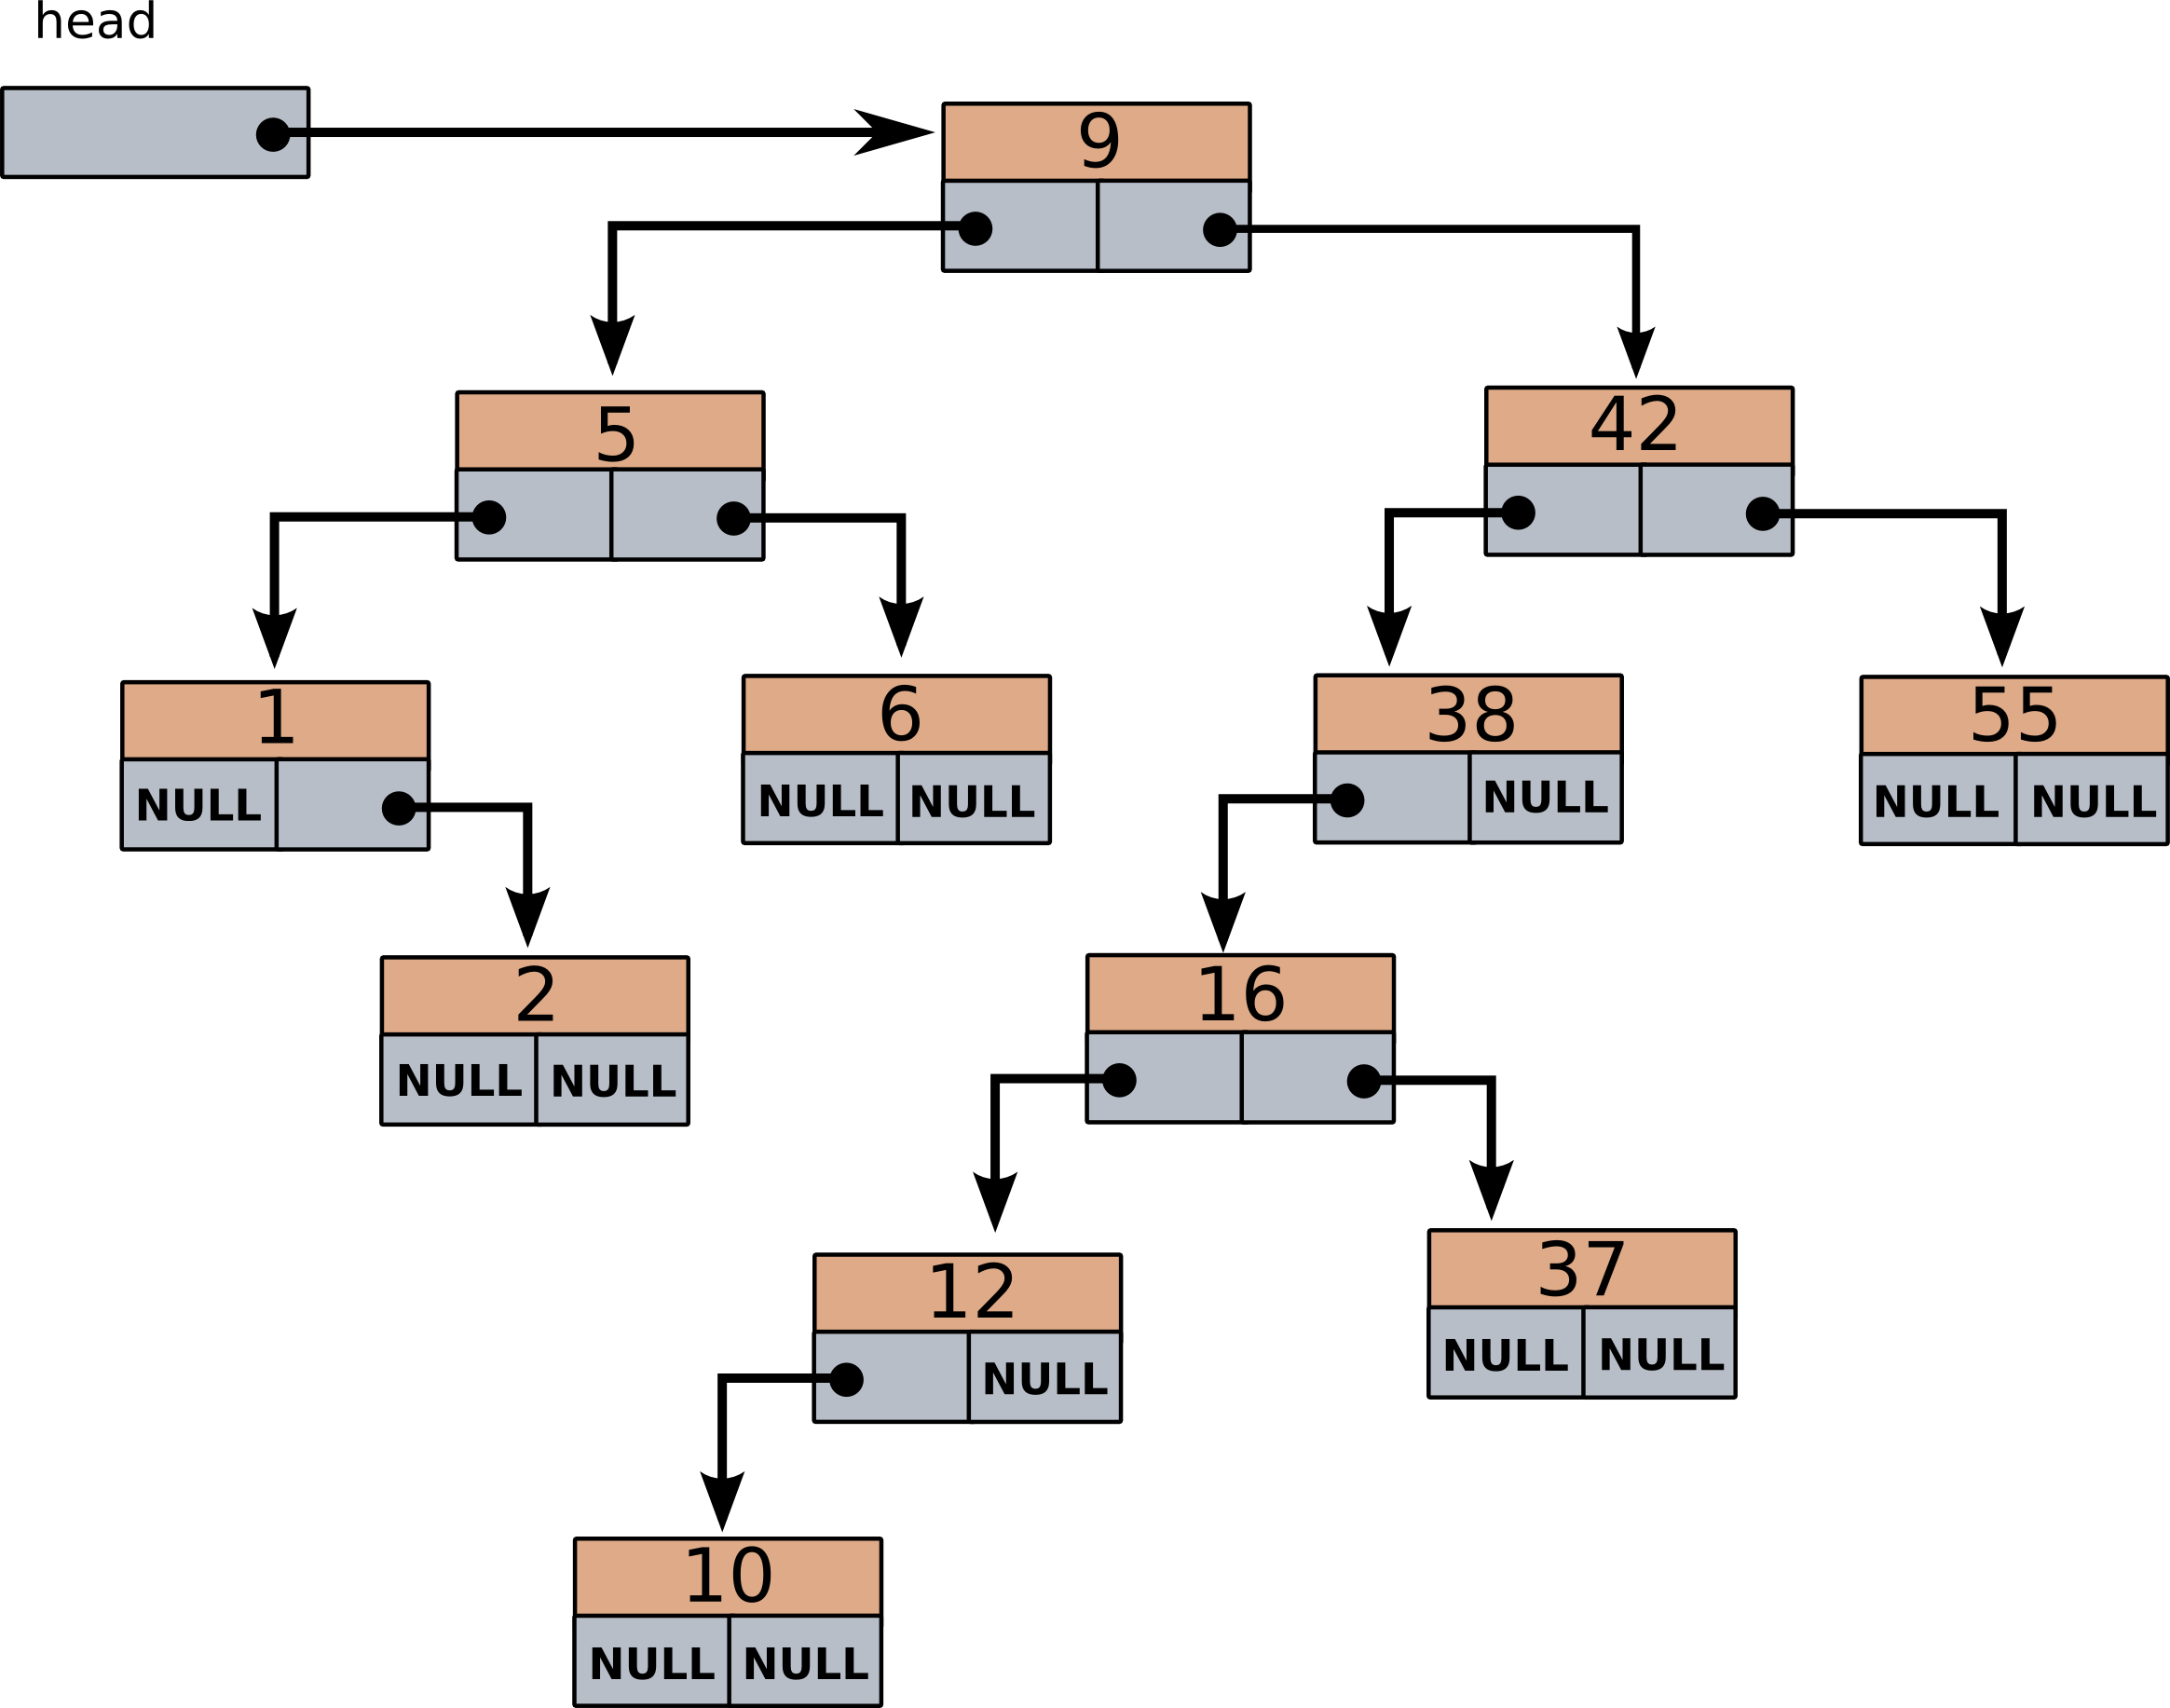
\includegraphics[width=0.96\linewidth]{../images/bintree_initial_1.png}
\end{center}
\end{multicols}

Бинарное дерево поиска это особый вид дерева, у которого для любого узла \texttt{ptr} выполняется следующее: 
\begin{itemize}
\item все значения левого поддерева меньше чем \texttt{ptr->val}
\item все значения правого поддерева больше или равны \texttt{ptr->val}
\end{itemize}

\subsection*{Задачи на бинарное дерево поиска}
\begin{enumerate}
\item Написать функцию \texttt{void binarytree\_insert(Node** p\_head, int val)}, которая добавляет элемент в бинарное дерево. Используйте цикл while для определения места добавления нового элемента.
\item Написать функцию \texttt{void binarytree\_insert\_rec(Node** p\_head, int val)}, которая добавляет элемент в бинарное дерево. Используйте рекурсию.
\item Написать функцию \texttt{int binarytree\_depth(Node* head)}, вычисляющую глубину бинарного дерева. Подсказка: напишите дополнительную рекурсивную функцию \texttt{int calculate\_binarytree\_depth(Node* ptr, int current\_depth)} и вызовите её из \texttt{binarytree\_depth}.
\item Решить задачу \textbf{data\_tree\_flat} из контрольной 2015/2016.
\item Написать функцию \texttt{Node* binarytree\_find(Node* head, int val)}, которая ищет элемент в бинарном дереве и возвращает указатель на этот элемент. Если такого элемента нет, то функция должна вернуть \texttt{Null}.
\item Написать функцию \texttt{Node* binarytree\_destroy(Node* head)}, которая освобождает всю выделенную память.
\end{enumerate}

\end{document}